\graphicspath{{chapters/5.Chapter_3/figures/}}

\begin{savequote}[75mm]
``All models are wrong, but some are useful''
\qauthor{- George E.P. Box \& Draper: \textit{Empirical model-building and response surfaces, 1987}}
\end{savequote}

\chapter{Metabolic integration}

\section{Introduction}

The linking of metabolism between host and endosymbiont is a fundamental 
stage in endosymbiotic integration \citep{Bhattacharya2007,Karkar2015a}.
Complementation of respective metabolic deficiencies/limitations in
host and endosymbiont allow exploitation of novel niches and provide
the key selective benefits of endosymbiosis \citep{Hoffmeister2003}.

In order to identify points of metabolic integration it is necessary to
identify the primary ``points of contact'' between the metabolic networks 
of host and endosymbiont. These ``points of contact'' comprise two
major classes of proteins, transporters and secreted proteins. 
Specifically, host and endosymbiont transporters which localise to the
perialgal vacuole (PV) membrane and the outer-membrane of the endosymbiont,
and proteins which are secreted by host and endosymbiont into 
PV.  

These points of contact can then be used to aid interpretation
and supplement inferred host and endosymbiont metabolic networks. 
By identifying these networks via the annotation and analysis of
assembled host and endosymbiont transcript complements it is putatively
possible to identify direct pathway integration.  For example,
the completion of a particular pathway via proteins derived from both
host and endosymbiont.

%Furthermore, comparison of networks derived from endosymbiotic
%species to previously sequenced genomes of 
%
%networks to 
%previously sequenced genomes from relatives of host and endosymbiont 
%such as \textit{P. caudatum} 
%and \textit{M. pusilum} NC64A can
%be used to identify possibly 

Finally, metabolic integration can be investigated by the 
direct analysis of metabolites.  This has the benefits of not
relying on abstracted measures such as transcript abundance or gene
copy to attempt to infer biological activity. By not treating the metabolic
state of the system as a latent variable novel information about the cellular
dynamics can be revealed.   For example, the existence of cryptic regulatory
systems that break-down direct mapping from genes to transcripts to protein to 
metabolites. By using both targeted and untargeted chromatography and mass
spectrometry metabolomics approaches it is possible to survey the combined
pool of host and endosymbiont both qualitatively and quantitatively. 
These inferences can then be correlated.

By utilising 3 separate streams of metabolic analysis, comparative transcript annotation
and mapping, directed identification and analysis of transporters and secreted
proteins and metabolomics, we maximise the strength of any inferences and 
reduce the chance of false negatives preventing the identification of biologically
important metabolic integration.

\subsection{Transporters}

The most important group of proteins in the control and evolution
of metabolic integration is that of host and endosymbiont transporter proteins.
This is due to their role in facilitating diffusion and active transport
across the lipid membranes that exist between host and endosymbiont.
While the role of transporters has been investigated extensively in 
several symbioses, these typically focus on organellar endosymbionts where
metabolic co-dependence has become fixed \citep{Yuan1994,Tyra2007,Huang2007,Li2010a} 
or ecological community interactions 
\citep{Richards2013,Hirner2006,Bachmann2013,Oldroyd2009}.


Without transporters many metabolically important 
large uncharged polar molecules (e.g. carbohydrates, amino acids)
and charged molecules (e.g. the various biologically relevant cations and anions such
as \(H^{+}\)) are incapable of significant rates of diffusion 
across membranes even in the presence of high concentration gradients. 
Therefore, the presence of transporters is vital to facilitating
any interaction involving these groups of metabolites. 
However, there are also several metabolites that are capable 
of unfacilitated diffusion across lipid membranes at significant rates.
These include important respiratory gases such as \(O_{2}\) and \(CO_2\),
hydrophobic compounds like benzene and small uncharged polar molecules
(e.g. \(H_2O\) and ethanol) \citep{cooper2013the,alberts2015molecular}.  
Despite this, transporter proteins have evolved to facilitate
even more rapid diffusion of some of these metabolites e.g. aquaporins
\citep{Agre1993}.  
Finally, transporters are important in that some can provide the ability
to actively transport metabolites against concentration gradients. 
This involves the expenditure of energy (typically in the form of ATP)
to directly pump compounds or generate an opposing gradient which can be
exploited (primary vs secondary active transport). 


There are 5 functional groups of transporters \citep{Saier2014}:
\begin{itemize}
    \item Channel/Pore types which catalyse diffusion of metabolites along concentration
        gradients e.g. porins and the Mitochondirla and Plastid Porin (MPP) family.
    \item Electrochemical Potential-driven transporters which use a carrier-mediated process to catalyse
        uniportation (single metabolite) or cotransportation (two species in the same
        direction, symportation, or two species in opposite direction, antiportation).  These make use
        of chemiosmotic gradients but generally do not directly make use of cellular energy molecules
        such as ATP. However, many make use of a gradient/potential generated by the active transport
        of solutes by another complex, in this case they can referred to as secondary active transporters.
        Electrochemical Potenital-driven transporters are a very large family and include 
        the ubiquitous major facilitator superfamily (MFS) and Cation Diffusion Facilitator (CDF) families. 
    \item Primary active transporters which use a direct source of chemical, electrical or light energy 
        such as ATP, voltage or photon to drive transport against concentration gradients.  Transporters
         of this type form many of the components fundamental to life as they allow an organism to 
         decouple itself directly from environmental and intracellular gradients. 
         They include rhodopsins, ATP-binding Cassette (ABC) Superfamily, and the general Secretory Pathway (Sec)
        family.
    \item Group translocators, which modify a substrate during transportation e.g. polysaccharide synthesis
        during secretion in the Polysaccharide Synthase/Exporter family and the Fatty Acid Group Translocation (FAT)
        family which can acylate fatty acids during transport.
    \item Transmembrane Electron Carriers which transport single electrons from a donor to an acceptor across
        a membrane. The major groups of these include the cytochrome and Photosystem I complexes. 
\end{itemize}

This analysis will primarily focus on transporters of the first 4 classes.
In the case of \textit{P. bursaria} and its endosymbiont we are
particularly interested in the host 
the host perialgal vacuole membrane and the outer membrane of the green
algal endosymbiont in the case of \textit{P. bursaria}.  
Therefore, the first step to the successful analysis of the metabolic
integration of host and endosymbiont is accurate identification of
transporter proteins present in their respective binned transcriptome
sequences.   By identifying both the identity of these proteins 
and qualitatively investigating the relative day:night expression
targets can be generated for further analysis, validation, and 
proof of localisation to the perialgal vacuole and algal outer
membrane.  Therefore, it is necessary to filter out 
transporters related to plastid and mitochondrial function in host and endosymbiont.

%The importance of these systems in metabolic integration is further 
%evidenced by the the way the evolution of protein import systems 
%from host to endosymbiont, such as the TICs/TOCs and TIMs/TOMs
%of plastids and mitochondria, is considered by many 
%to be the main constraint in the establishment of an endosymbiont
%as an organelle \citep{Pfanner2001.Keeling2008a}.


Transporter proteins can be predicted  
primarily via annotation and homology searches to previously
identified transporters \citep{Saier2006,Saier2009,Saier2014} 
and direct identification of transmembrane (TM) domains motifs. 
All transporters feature at least 1 TM helix, usually considerably
more \citep{VonHeijne2006}.  However, as not necessarily every sub-unit of
a transporter will contain a TM domain and the presence of partial transcripts
in our assemblies it is necessary to not rely totally on TM prediction to discover
transporter proteins.

One obvious target of such an analysis is based on the most obvious point
of metabolic integration between a host and its photosynthetic endosymbiont.
The exchange of photosynthate and the provision of a nitrogen source.
Specifically, we wish to discover sugar transporters which facilitate the
secretion and uptake of photosynthate and ammonium and/or amino acid transporters
which facilitate transfer of a nitrogen source between host and endosymbiont.

\subsection{Carbohydrate Metabolism}

%Since their discovery \citep{Cohen1957}, several functional types of transporter proteins have been identified:
%uniporters which facilitate transfer along the sugar gradient (e.g. hexose
%transporter (HXT), glucose-transporter (GLUTs), and SWEETs),
%and cotransporters which couple transport to another gradient. 
%Co-transporters are further divided into symporters such as sodium-glucose symporters (SGLTs), sucrose-\(H^{+}\) 
%cotransporter (STP), and SUT which co-transport cations in the same direction and
%antiporters such as the tonoplast sugar transporter (TST) that uses opposing
%gradients \citep{Chen2015}.

The transfer of matlose, glucose, fructose and malate from endosymbiont
to host has been observed using radiolabelling 
\citep{Brown1974}.  Furthermore, green algae strains competent to
form endosymbioses were found to inducibly release significantly
more photosynthate (in the form of \(\sim 95\%\) maltose) than strictly free-living strains
in the presence of \(NaHCO_3\) on the order of \(5.4-86.7\%\) vs. \(0.4-7.6\%\)
of total photosynthate \citep{Muscatine1967a}.

In terms of the uptake of saccharides, \textit{C. vulgaris} (the current
taxonomic state of this strain is unclear) has an inducible system for active hexose uptake \citep{Tanner1974}.
Additionally, studies in the Japanese \textit{C. variabilis} endosymbiont strains
indicates some lack the capability to directly utilise sucrose or maltose in free-living culture \citep{Kamako2005}
as well an inability to import glucose or fructose \citep{Kato2008a} (although glucose and maltose
did stimulate growth \citep{Kamako2005} it was via a different mechanism \citep{Kato2009}.

There are 3 main groups of eukaryotic sugar transporters in the green algae: 
major facilitiator superfamily (MFS) transporters including glucose
transporters (GLUTs), HXTs, STPs and SUTs; the Sodium-Solute Symport Family (SSF) sodium-glucose symporters (SGLTs); 
and SWEETs \citep{Chen2010a,Chen2015}.
Additionally, there are a few transporters mainly associated with intracellular transport such as 
vacuolar glucose transporter I (VGT1), ERD-like transporters and tonoplast monosaccharide transporters.

Therefore, this analysis of sugar transporters will feature both general screening
for transporters as well as targeted homology searches for elements of these
transporter families.

\subsection{Nitrogen Metabolism}

Nitrogen is the most transferred material between host and endosymbiont
after carbon \citep{Kato2009}.  There has been considerable research and interest
in exactly what form this nitrogen exchange takes place.


In terms of nitrogen utilisation in endosymbiotic algae 
\textit{C. variabilis} both NC64A and F36-ZK demonstrated an ability
to effectively use amino acid, less effectively use ammonium and not
use nitrate or nitrite \citep{Kamako2005,Kato2009}.
European endosymbionts (now mostly renamed to \textit{M. reisseri}) display
a similar pattern but have 
shown an ability to use nitrate as well \citep{Kessler1990}.
This is in contrast to obligately free-living species such as \textit{Parachlorella
kessleri} which can make use of all the above nitrogen sources \citep{Kato2009}.


As \textit{P. bursaria} cannot import nitrate \citep{Albers1982} the heterogeneous
loss of nitrate and nitrite utilisation in endosymbiotic strains is perhaps not surprising \citep{Kato2009}.
As there is no pressure to maintain enzymes necessary for this pathway when an endosymbiont
this may explain the appearance 

This reduced selection pressure for nitrate and nitrite utilisation when in the endosymbiot
milieu may explain the presence of low-activity mutatant Nitrate Reductase (NR) and Nitrite
Redutase (NiR) \citep{Kato2009}. 
Putatively, this reflects an early stage in the genomic streamlining that frequently
takes place in endosymbionts. 


A study of specific amino-acid utilisation identified
6 amino acids that promited strong growth L-arginine, L-asparagine,
L-glutamine, L-serine, L-alanine in \textit{C. variabilis} F36-ZK \citep{Kato2006}.
There was also no growth observed with the dipetptides
glycylglycine, glycyltyronsine, and arginlyarginine \citep{Kato2006}.

A similar but much earlier study in \textit{C. variabilis} NC64A
showed use of L-arginine, L-glutamine and L-lysine although L-arginine wasn't
found to be actually imported \citep{McAuley1986}.  A similar




L-glutamine and L-glutamic acid

k






 Respiration of the host plays a role in the gas exchange of \(CO_2\) and \(O_2\) 
 to the endosymbiont, with the algae displaying higher levels of photosynthetic
 activity while in association with the host due to the increase host related 
 \(CO_2\) respiration \citep{Reisser1980}.
Addition of glucose, which likely increases host respiration rate and thus \(CO_2\)
evolution increases the rate of photosynthetic oxygen production commensurately \citep{Reisser1980}




Proton gradient dependent transport of maltose/photosynthate out of the \citep{Schussler1992}
pH induces release of maltose in many algae \citep{}

%In \textit{Parachlorella kessleri} (previous \textit{Chlorella kessleri} \citep{Krienitz2004,Hoshina2010})
%
%Chlorella \(H^{+}\)-monosaccharide (HUP1) co-transporters \citep{Sauer1989}
%have been identified (via hexose-transport deficient mutant screens \citep{Sauer1986}
%and localised to the plasma membrane \citep{Stadler1995}
%Additionally these transporters have been identified in the
%\textit{Auxenochlorella protothecoides} (formerly \textit{Chlorella protothecoides} \citep{Champenois2014}) genome \citep{Gao2014}.


\subsection{Secreted proteins}

The next major class of proteins involved in endosymbiosis
from the perspective of the endosymbiont as those
which are secreted.   These proteins are secreted
into the perialgal vacuole and thus are likely to
be play some form of role in the maintenance of
the endosymbiosis.


Identification of secreted proteins also offers
a chance to further elucidate the function of novel or poorly 
characterised transporters that have been identified. 
For example, 

Secreted proteins can be effectively identified by 
searching for the presence of N-terminal signal peptides. 

These are short 15-30 amino acid N-terminal sequences cleaved during translocation.
They aren't conserved sequences but are present across the tree of life.

Feature a biochemical compositional fingerprint 
of positively charged residues, hydrophobic residues and polar uncharged
residues with distinctive points before site.l \citep{Emanuelsson2007}





Not all have signal peptides either





SignalP \citep{Nielsen1997} has proven the most effective method of predicting
the presence of signal peptides \citep{Lee2009a,Petersen2011}.


This method uses a standard feed-forward artificial neural network
with 8-41 hidden units (depending on whether the organism is eukaryotic, 
gram positive or gram negative) trained with back-propagation.




By analysing the identified signal peptides it is possible
to 

\subsection{Metabolic mapping}

Metabolic pathways form the functional backbone of all biological processes. 
The Kyoto Encyclopedia of Genes and Genomes (KEGG) \citep{Ogata1999,Okuda2008,Kanehisa2014} 
and MetaCyc \citep{Caspi2007} databases form an important resource for contextualising
genomic and transcriptomic scale results into these networks. 
The utility of this approach is emphasised by the presence of numerous
tools and analytical pipelines to explore these databases 
e.g. \citep{Okuda2008,Nakao1999,Karp2002,Karp2010,Antonov2008,Klukas2007}

By comparison of the relatively complete predicted peptides from 
the endosymbiotic algae \textit{C. variabilis} NC64A and \textit{Coccomyxa
subellipsoidea} C-169 genome projects to the predicted endosymbiont binned peptides
from the transcriptomes of \textit{M. reisseri} and \textit{C. variabilis} 1N
it is possible to infer what the endosymbiotic metabolic pathways
are active during endosymbiosis. 













what metabolic pathways are likely










\subsection{Metabolomics}


A pilot untargeted global metabolomic profile was generated
for \textit{P. bursaria}-\textit{M. reissieri} CCAP 1660/12 
culture to test the feasability of this approach and help optimise
chromatography and 

Finally, a proof of concept for the targeted metabolomic
analysis of this system was conducted used HPLC-QQQ
to determine the relative abundances of amino acids
in the culture between day and night conditions. 

In the case of \textit{P. bursaria} and its green algal endosymbionts 
there are



\subsubsection{Untargeted Global Profiling}
GCMS, LCMS,

\subsection{Targeted Analysis of Key Classes of Compounds}

Mass spectrometry also offers methods by which a targeted 
analysis of key classes of compounds can be conducted. 


While few

Amino acids 



\section{Aims}

The principal aim of this chapter is to identify
likely points of metabolic integration between host and 
endosymbiont to generate targets for subsequent 
targeted mass spectrometry, RNAi and qPCR based validation
experiments. 

This will be achieved by:
\begin{itemize}
\item identifying
    transporter proteins present in the endosymbiont
    binned transcripts from the CCAP1660/12 RNA-Seq analysis
    and analysing them for qualitative differential 
    expression between day and night. 
\item identifying
    secreted proteins present in the endosymbiont
    binned transcripts from the CCAP1660/12 RNA-Seq analysis
    and analysing them for qualitative differential 
    expression between day and night. 
\item Comparative analysis of metabolic pathways 
    between host and endosymbiont relative to 
    sequenced green algal genomes. 
\item A pilot untargeted global metabolomic profile of the 
    system and comparison of day to night.
\item Targeted quanitative analysis of amino acid concentrations
    between day and night. 
\end{itemize}

\section{Methods}
\subsection{Transporter Analysis} 
\subsubsection{Transporter identification pipeline}
Transporters were identified in the 4 sets of sequences (\textit{C. variabilis}, \textit{M. reisseri},
\textit{C. vulgaris} and \textit{C. subellipsoidea}) using the following set of pipelined filters:
\begin{enumerate}
    \item Transmembrane (TM) domains were predicted for each sequence using an HMM approach implemented as part of TMHMM2 \citep{Sonnhammer1998,Krogh2001}
and sequence predicted to contain at least 1 TM domain was extracted.
    \item These sequences were then used to search a PFAM database of profile HMMs \citep{Eddy1998} via HMMER3's hmmscan utility \citep{Eddy1995,Johnson2010,Eddy2011,Mistry2013}
        and sequences with a hit to a PFAM domain at an independent E-value of \(1e^{-5}\) were retained.
    \item These hits were then finally filtered for PFAM domains which mapped to transporter families classified by the Transporter Classification Database (TCDB) \citep{Saier2006,Saier2008,Saier2009,Saier2014}
        mapping files.
\end{enumerate}

Additionally, to ensure thorough discovery of 
all \textit{M. reisseri} transporters \textit{M. reisseri} binned sequences 
were BLASTP-ed against the NR protein database with an e-value of \(1e^{-3}\) and 20 hits.
InterproScan \citep{Zdobnov2001a} was then used to 
further annotate these proteins incorporating
results from BlasProDom \citep{Servant2002}, FPrintScan \citep{Attwood1994}, 
HMMER \citep{Eddy2001} scans against the PIR \citep{Barker1998}, PFAM \citep{Bateman2002}, 
SMART \citep{Schultz1998}, PANTHER \citep{Thomas2003a} and TIGRFAM databases \citep{Haft2003}, 
ProfileScan \citep{Gribskov1988},
HAMAP \citep{Lima2009}, PatterScan, 
SuperFamily \citep{Gough2002}, 
SignalP \citep{Petersen2011}, TMHMM \citep{Sonnhammer1998}, 
Gene3D \citep{Buchan2002}, Phobius \citep{Kall2007}
and Coils. Results were then mapped to GO terms \citep{Ashburner2000,Harris2004}
and annotated via BLAST2GO \citep{Conesa2005a}.

Finally, all proteins annotated to have a GO term associated with ``transport'' and
``transport activity'' specifically, GO:0005215, GO:0005478 and GO:0006810 and their child
terms were extracted.  

\subsubsection{Qualitative expression analysis}

Kallisto \citep{Bray2015} was used to pseudoalign and estimate abundances for 
all taxonomically screen single cell 
libraries (4 dark and 3 light) to the called ``endosymbiont''
binned CDS sequences from the \textit{P. bursaria} CCAP 1660/12
transcriptome (see Chapter 2).

Kallisto doesn't align reads to references in the same
manner as conventional short read alignment algorithms
such as Bowtie2 \citep{Langmead2012}.  Instead of specifically 
mapping a read to a set of co-ordinates it instead
determines which transcripts are compatible with the alignment 
of a given read.  This is achieved via decomposition of transcripts
in de-Bruijn graphs and fast k-mer hashing to compare reads to transcript
graph nodes in constant time.  These k-compatability classes are then used with
boostrapped expectation-maximisation to estimate transcript quantification and
determine uncertainty \citep{Bray2015}. 

Results were visualised and analysed using ``sleuth'' and the
seaborn plotting library \citep{michael_waskom_2015_19108}.

\subsection{Secretome prediction}

A conservative set of secreted proteins were predicted 
using the following pipeline:
\begin{enumerate}
    \item Signal peptides are detected using SignalP4.1 and mature sequences
        created for each sequence with a signal peptide
    \item Sequences detected to have a TM domain (by TMHMM) within either the mature sequence or 
        full length for proteins without signal peptides were discarded.
    \item Signal peptides were re-added to mature sequences and the 
        remaining sequences were then filtered using for those predicted as secreted by TargetP1.1 
    \item These sequences were then filtered down to those which had extracellular
        localisation in WoLFPSORT 0.2 
    \item Finally, for the endosymbiont, secreted protein found to have a Chloroplast
        targeting signal (via ChloroP1.1) were removed.
\end{enumerate}

\subsection{Metabolic mapping analysis}

First, predicted proteomes were obtained or generated for
\textit{Coccomyxa subellipsoidea} C-169, \textit{Chlorella variabilis}
NC64A, \textit{Chlorella variabilis} 1N, and \textit{M. reisseri}. 

For \textit{M. reisseri} the endosymbiont binned sequences from the transcriptomic
sequencing project discussed in the previous chapter were used. 
\textit{Coccomyxa subellipsoidea} C-169 genome project \citep{Blanc2012} version 2.0 
JGI annotated proteins (created 12-01-2014) were downloaded from JGI's
Phyotozome v10.3.1 \citep{Goodstein2012}. 
Similarly, the ``best'' annotated proteins from
version 1 of the \textit{Chlorella variabilis} NC64A genome project \citep{Blanc2010}
were downloaded from JGI's genome portal \citep{Grigoriev2011,Nordberg2014}

However, to obtain \textit{C. variabilis} 1N endosymbiont peptides 
a reassembly and binning of raw sequencing data from \citep{Kodama2014}
was conducted (discussed below). 

Once all sequences were acquired they were annotated using KEGG
orthology.  This was achieved 
using the KEGG Automatic Annotation Server (KAAS) \citep{Moriya2007a}
single-directional best hit with both BLAST and GHOSTZ \citep{Suzuki2014,Suzuki2015} 
method against the following 40 gene sets: \textit{Homo sapiens}, 
\textit{Drosophila melanogaster}, \textit{Caenorhabditis elegans},
\textit{Arabidopsis thaliana}, \textit{Gylcine max},
\textit{Vitis vinifera}, \textit{Oryza sativa}, 
\textit{Ostreococcous lucimarinus}, \textit{Ostreococcus tauri},
\textit{Micromonas} sp. RCC299, \textit{Cyanidioschyzon merolae},
\textit{Galdieria sulphuraria}, \textit{Saccharomyces cerevisiae},
\textit{Candida albicans}, \textit{Neurospora crassa}, \textit{Aspergillus nidulans},
\textit{Coccidioides immitis}, \textit{Schizosaccharomyces pombe},
\textit{Ustilago maydis}, \textit{Encephalitozoon cuniculi},
\textit{Monosiga brevicollis}, \textit{Dictyostelium discoideum}, 
\textit{Acanthamoeba castellanii}, \textit{Plasmodium falciparum} 3D7, 
\textit{Cryptosporidium hominis}, \textit{Tetrahymena thermophila},
\textit{Paramecium tetraurelia}, \textit{Phaeodactylum tricornutum},
\textit{Emiliania huxleyi}, and \textit{Guillardia theta}.

KEGG annotations were then plotted onto KEGG metabolic networks and compared 
to identify key aspects of differences between the algal species and
host and endosymbiont metabolic.

\subsubsection{\textit{Chlorella variabilis} 1 N assembly}
\(232.3M\) 100bp paired-end reads from \citep{Kodama2014}'s 
bulk RNAseq transcriptome of \textit{Paramecium bursaria} Yad1g (syngen
3, mating type 1) bearing \textit{Chlorella variabilis} 1N endosymbionts
were downloaded from the DNA Data Bank of Japan (DDBJ) \citep{Tateno2002,Kaminuma2011}
in Sequence Read Archive (SRA) format \citep{Leinonen2011,KodamaNRA2012b} (accession DRA000907 \citep{Kodama2014}).

These reads were then converted to fastq using ``fastq-dump'' using the SRA Toolkit
\citep{NationalCenterforBiotechnologyInformation2011}.  Reads were then trimmed
for sequencing adapters using ILLUMINACLIP and SLIDINGWINDOW with a window size
of 4 and a minimum average quality of 5 in Trimmomatic \citep{Bolger2014a}.

Reads were then error-corrected using ``SEECER'' with a k-mer size of 25 and 
default settings otherwise (entropy of 0.6 and a cluster log-likelihood
of -1) \citep{Le2013}.  Error-corrected reads were digitally normalised
using a K-mer size of 25 and a coverage of 20 \citep{Brown2012} and 
low abundance K-mers in high coverage reads were filtered \citep{Zhang2014,Zhang2015}
using the Khmer software package \citep{Doring2008,Crusoe2015}.

Assemblies were completed in a modified/fixed version of 
Bridger 2014-12-01 \citep{Chang2015} (available at
\url{https://github.com/fmaguire/Bridger_Assembler}) and 
Trinity v2.0.6 \citep{Grabherr2011,Haas2013} both with K-mer
sizes of 25.

An alternative Trinity assembly was also completed using
SLIDINGWINDOW Q30 trimmed reads without normalisation or 
error correction.

Assemblies were then compared using RSEM-EVAL \citep{Li2014} and the best
overall assembly selected on the basis of likelihood.

ORFs were called from the best assembly using universal and tetrahymena encodings 
via TransDecoder \citep{Haas2013} retaining the best scoring sequences and those
with HMMR hits to PFAM and BLASTP hits to the swissprot database. 

Phylogenies were generated for each sequence using the same approach and pipeline
described in Chapter 2. These phylogenies were subsequently classified using the 
same trained K-Neighbours supervised learning algorithm.
Any sequence that didn't have enough BLAST hits in the genomes used to generate
a phylogeny (5) were parsed based on what hits were retrieved.
Those with no hits were classified as ``unknown'' and those with
hits were classified based on the origin of those hits e.g. hits
to green algae and plant genomes were considered ``endosymbiont'' and so on.

Finally, the ORF bins for host and endosymbiont 
from both encodings were manually combined and reconciled
to generate transcript bins.  With the transcripts binned into
``host'' and ``endosymbiont'' ORFs were recalled from them using the appropriate
encodings. 




\subsection{Metabolomics}

3 mass spectrometry analyses were conducted to investigate the presence/absence
and relative abundances of polar and non-polar metabolites.

Finally, a targeted mass spectrometry analysis was conducted using
LC-QQQ to quantitatively assess 



\subsubsection{Untargeted LC-QTOF Profiling}

Sample preparation for mass spectrometry followed standard protocols.
Briefly, 5 biological replicates were sampled from \textit{P. bursaria} CCAP 1660/12 
cultures at the midpoint of both the day and night cycles. 
Samples were then dried, flash-frozen in liquid nitrogen, and homogenised
using a cell disruptor. 

For each sample, \(10mg\) was dissolved in \(400\mu l\)
of a solution of \(80\%\) MeOH containing \(7.2mg ml^{-1}\) of
an umbellifrone internal standard.  This solution was kept on ice
and vortexed for 30s every 10 minutes for 30 minutes.
Samples were sonictated in ice cold water for 15 minutes and then centrifuged
at 13k rpm for 10 minutes.  Retaining the supernatant in a separate tube, the pellet
was resuspended in \(400\mu l 80\%\) MeOH and vortexing, sonication and centrifugation
steps repeated.  The two supernatants were combined and filtered through 
a \(0.2\mu m\) syringe filter (Chromacol).  Samples were sub-divided into two 
a \(5\mu l\) of each was loaded into an Agilent 1200 Series HPLC with
a \(3.5\mu m\), \(2.1\times 150mm\) Eclipse Plus C18 Agilent column.
One sample was then analyses using a positive electron spray ionisation
and the other a negative ionisation on an Agilent 6520 accurate mass
quadrupole time of flight (Q-TOF) mass spectrometer. Data was captured
using the standard Agilent data acquisition software and converted
from ``.d'' format to the open mzXML format \citep{Pedrioli2004}.
The same process was repeated for 7 blank samples under both ionisation conditions
as well as an apigenin QC standard.

Samples were analysed primarily using the XCMS R package \citep{Smith2006,Tautenhahn2012}.
Peak features were detected in each samples using the centWave algorithm with a 30ppm tolerated m/z deviation,
minimum peak width of 10 and maximum peak width of 60 \citep{Tautenhahn2008}. 
Peaks were aligned with a 0.025 m/z width overlap, and a maximum bandwidth 5 retention time
deviation. Using the aligned peaks, the retention time deviation between samples were
calculated.  The samples were then realigned correcting for retention time deviation and
integrated using fillPeaks. 

In order to determine differential presence of globally detected metabolites
unpaired Welch's \textit{t}-tests were conducted comparing the 5 day samples to the 5
night samples. Welch's tests were used as they don't assume equal sample sizes or variances
between the two groups\citep{Welch1947}\footnote{
    \(t' = \frac{\mu_1 - \mu_2}{\sqrt{\frac{s^2_1}{n_1} + {s^2_2}{n_2}}}\)
    with degrees of freedom determined via the Welch-Satterwaite-equation:
    \(df = \frac{(\frac{s^2_1}{n_1} + \frac{s^2_2}{n_2})^2}{\frac{(\frac{s^2_1}{n_1})^2}{n_1 - 1} + \frac{(\frac{s^2_2}{n_2})^2}{n_2 - 1}}\)
    \citep{Ruxton2006}
}

P-values from this were corrected 
for multiple comparisons using false discovery rates (FDR).  FDR is a
less conservative correction than, the classic family-wise error rate correction,
Bonferroni adjustment\footnote{
    P-value threshold \(\alpha\) is adjusted relative to the number of comparisons (n). 
Specfically, significance is determined as a P-value \(\leq \frac{\alpha}{n}\).} but
allow maintenance of a greater proportion of statistical power with a 
slightly evelated risk of Type-I errors. 

Features were then annotated using the METLIN metabolite database \citep{Smith2005a,Sana2008,Tautenhahn2012a}.
Extracted ion base peak chromatograms were manually inspected for each significantly expressed feature
and any that weren't clear distinct peaks were discarded. Any sample without
an annotation against METLIN was similarly discarded. Finally, annotations
were manually parsed and samples with impossible annotations (e.g. 
chemotherapeutic drugs) discarded.  

\subsubsection{Untargeted GC-QTOF Profiling}

%heoretically, GC-QTOF would ideally be used to identify profiles of polar
%saccharides. 

%Pseudospectrum approach instead of peak alignments etc due to the difficulties
%aligning data of this type relative to LCMS.
%
%Peak picking followed by pseudospectra determination.
%Identification and elemeiaton of artefacts and then annotation
%against a standards database. 
%
%Rather than individual peaks - a pseudospecvtrum is used.
%This is a set of m/z values with a peak at the same rentetion time.
%In GC the overalp is smaller than in LC due tot he narrower peaks therefore
%retention times are harder to match leading to separate mass spectra. 
%
%NIST library has fragmentation patterns.
%
%Spectra are easier to interepr due to adducts - 
%
%Comparison of pseudospectra is done via a weighted dot product
%
%Finally unannotated patterns repeatedly occur in different 
%
%LC-QTOF was conducted using

%abd were charged using dual electronspray ionisation (ESI), one run
%using a negative polarity and the other positive. 
%
%\(3.5\mu m\), \(2.1 \times 150mm\) Eclipse Plus C18 (Agilent) 

\subsubsection{Targeted Amino Acids Quantitative Analysis}

5 Day and 5 Night samples were prepared for liquid chromatography
using the same approach as the untargeted LC-QTOF analysis.
In addition to this, the Day1 and Night1 samples were analysed at both
\(2x\) and \(0.5x\) titrations.  3 blank samples were run 
as well as standards consisting of a complete amino acid
mix from Sigma at \(0.5\mu M\) and 4 samples consisting of Asparagine-Glycine-Tryptamine
and Leucine-Glutamine-Lysine respectively.

After chromatography samples were ionised using electronspray ionisation
and analysed using multiple reaction monitoring optimised
for amino acids with an Agilent Technology
6410B enhanced sensitivity triple quadrupole mass spectrometer (QQQ).

Results were analysed using the Agilent Quantiative Analysis software package
with peaks normalised in respect to the umbelliferone standard.  Results for any 

















Agilent 6410 enhanced sensitivity triple quadrupole (QQQ) 
with Agilent 1200 series HPLC stack





\section{Results}

\subsection{Kodama Assembly}

\begin{table}
    \centering
    \begin{tabular}{|c|c|}
        \hline
        \textbf{Preprocessing} & \textbf{PE Reads} \\
        \hline
        \textbf{Raw Reads}  & \(2.323\cdot10^{8}\)\\
        \textbf{Q30 Trimmed} & \(1.75\cdot10^{8}\)\\
        \textbf{Q5 Trimmed}  & \(2.127\cdot10^{8} \) \\
        \textbf{Q5 Error Corrected}  & \(2.021\cdot10^{8}\)\\
        \textbf{Q5 Digital Normalistion} & \(1.09 \cdot10^{7}\)\\ 
        \textbf{Q5 K-mer abundance filtering} & \(1.055\cdot10^{7}\)\\
        \hline
    \end{tabular}
    \caption{Summary of read pre-processing stages for tthe Kodama library demonstrating
    the massive amount of redundancy that digital normalisation removes from the assembly.
The low amount number of reads removed during K-mer abundance filtering indicates
that there were relatively few low abundance 
}
    \label{tab:kodama_preproc}
\end{table}

\begin{table}
    \centering
    \begin{tabular}{|c|c|c|}
        \hline
        \textbf{Assembly} & \textbf{Contigs} & \textbf{Likelihood (\(-log\))}\\
        \hline
        \textbf{Trinity Q5 Normalised}  & 101,957 & \(1.216\cdot10^9\)\\
        \textbf{Bridger Q5 Normalised} & 62,504 & \(1.285\cdot10^9\)\\
        \textbf{Trinity Q30} & 53,938  & \(5.619\cdot10^{9} \) \\
        \hline
    \end{tabular}
    \caption{Summary of Kodama assembliesj}
    \label{tab:kodama_assembly}
\end{table}

Therefore, the optimal assembly chosen for further analysis was the Trinity
Q5 normalised assembly on the basis of RSEM-EVAL score. 

From the 101,957 transcripts 193,906 ORFS were called using tetrahymena 
encoding and 20,875 universal.

These were subsequently binned using the same approach as used in 
Chapter 3. 

\begin{table}
    \centering
    \begin{tabular}{|c|c|}
        \hline
        \textbf{Bin} & \textbf{Number of Transcripts} \\
        \hline
        Food & 3,873 \\
        Endosymbiont & 8,627 \\
        Host & 53,295 \\
        Unknown & 36,162 \\
        \hline
    \end{tabular}
\end{table}

Finally, ``Host'' and ``Endosymbiont'' binned transcripts 
were re-ORF called using the appropriate encodings to result in a 
host ORF bin of 61,239 sequences
and an endosymbiont bin of 5,565 peptides. 

\subsection{Transporter Identification}

To identify transporters present in the translated protein dataset of the 
endosymbiont bins of the CCAP1660/12 and YADGN1 
\textit{Paramecium bursaria} transcriptome assemblies, as well as the Chlorella NC64A 
and Coccoymxa C-169 predicted proteomes the following process was used:

\begin{table}
    \centering
    \begin{tabular}{|c|c|c|c|c|}
        \hline
        & \textit{C. variabilis 1N} & \textit{M. reisseri CCAP 1660/12} & \textit{C. vulgaris NC64A} & \textit{C. subellipsoidea C-169} \\
        \hline
        Peptides        & 5,565 & 4,275 & 9,791 & 9,629 \\
        1+ TM domains   & 695 & 419 & 1,722 & 1,709 \\
        1+ TM and TCDB  & 251 & 185 & 690 & 697 \\
        \hline
    \end{tabular}
\end{table}






A set of 233 
transporter proteins were also identified 
in the \textit{M. reisseri} binned peptides
by parsing the results of a 
BLAST/InterProScan and GO term based annotation pipeline.
Of, these 77 were redundant to proteins already identified using
the TM/TCDB pipeline, therefore 156 were novel.

This means a total of 341 transporters were identified 
belonging to the CCAP 1660/12 endosymbiont from the SCT transcriptomes. 







\begin{figure}
    \centering
    \includegraphics[width=\textwidth]{endosymbiont_bin_annotation.pdf}
    \caption{More stringent} 
\end{figure}



\begin{figure}
    \centering
    \includegraphics[width=\textwidth]{endo_distribution_of_top_BLAST_hits.pdf}
    \caption[Endostymbiont Bin Top BLAST Hits]{asdasd}
\end{figure}


\begin{figure}
    \centering
    \includegraphics[width=\textwidth]{endosymbiont_bin_size_dist.pdf}
    \caption{asdasd}
\end{figure}






\subsection{Kallisto quantification analysis}

Using the nucleotide CDS sequence of the called peptides identified as transporters
from the primary SCT transcriptome. 

Due to the compositional/coverage biases of MDA-based single cell transcriptomics 
Kallisto statistical inference was likely to be spurious and relate to the 
well-documented coverage biases of MDA. Therefore, a simple presence/absence
filter was implemented for the single cell libraries where an estimated
Transcripts per million (TPM) was above 0 for at least 1 biological replicate
in each condition. 
TPM is an estimate of the 

\begin{figure}
	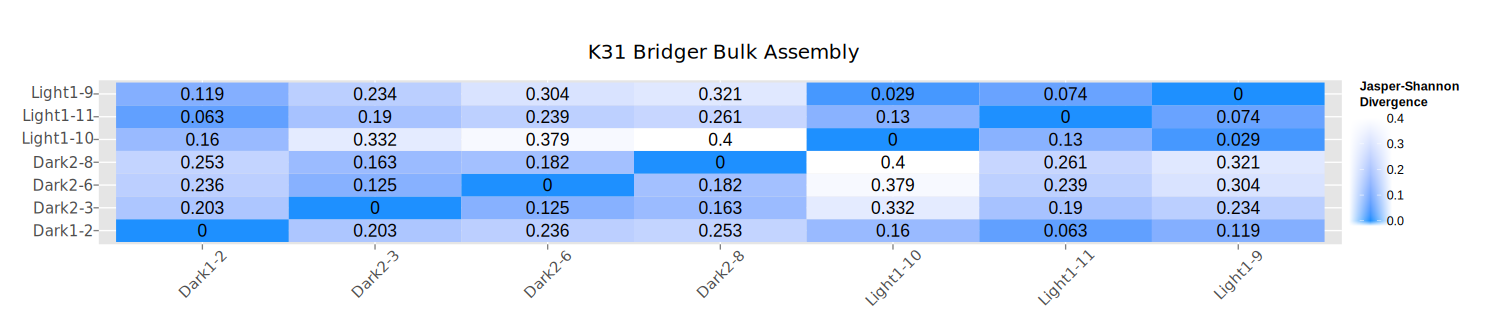
\includegraphics[width=\textwidth]{bjsvg.pdf}
    \caption[Jasper-Shannon Divergence of Single Cell Libararies]{Comparison of single cell libraries}
\label{fig:jsd}
\end{figure}


% \begin{figure}
%     \includegraphics[width=\textwidth]{transporter_expression_heatmap.pdf}
%     \caption{A binary filter heatmap that displays the 4 groups of transporter
%         proteins identified in the \textit{P. bursaria}-\textit{M. reisseri} 
%         transcriptome.  Specifically, it shows 33 transporters expressed only
%         in the dark single cell libraries, 54 expressed only in the light,
%     84 expressed in both libraries and 13 only recovered in the bulk transcriptomes}
%     \label{fig:binary_expression_heatmap}
% \end{figure}


Of these only 2 were expressed in all 4 bulk libraries 34 in all 3 light libraries, 14 in all taxonomicall screened SCT libraries.

\begin{table}
    \begin{tabular}{|c|c|c|c|}
        \hline
        \textbf{State} & \textbf{Name} & \textbf{TCDB Identity} & \textbf{TCDB Annotation}\\
        \hline
        All Dark Libraries  & comp11781\_seq0|m.10145 & PF00448.18 & General Secretory Pathway \\
                            & comp20734\_seq0|m.20988 & PF00122.16 & P-type ATPase \\
        \hline
        All Light Libraries & comp34406\_seq1|m.34111 & PF02705.12 & K+ potassium transporter/Drug-Metabolite Transpoter/K+ uptake permease\\
                            & comp55761\_seq0|m.51120 & PF07690.12 & Major Facilitator Superfamily \\  % GPH:cation symporter ATP:ADP antiporter family -MFS CAN DO SUGAR
                            & comp26454\_seq0|m.27109 & PF03239.10 & Iron permease FTR1 family  \\
                            & comp12997\_seq0|m.11462 & PF02653.12 & Brnached-chain amino acid transport system/permease/ATP-binding cassette\\
                            & comp2196\_seq0|m.2436   & PF00361.16 & Proton-conducting membrane transporter, H+/Na+ translocating NADH dehydrogenase family, monovalent cation (K+/Na+): Proton antiporter-3 \\
                            & comp30376\_seq0|m.30648 & PF01490.14 & Transmembrane amino acid transporter, MFS/Amino acid/auxin permease\\
                            & comp8796\_seq0|m.7077   & PF01241.14 & Plant Photosystem 1 Supercomplex (psaG/psaK) \\
                            & comp16529\_seq0|m.15912 & PF00032.13, PF00033.15 & Cytochrome b (PRC) \\
                            & comp39264\_seq0|m.37815 & PF01970.12 & Tripartite tricarboxylate transporter (TctA) \\
                            & comp12686\_seq0|m.11025 & PF01970.12 & TctA family  \\
                            & comp18033\_seq0|m.17793 & PF03401.10 & TctC family \\
                            & comp16603\_seq1|m.16010 & PF00860.16 & Permease (CDF) \\
                            & comp1093\_seq1|m.1645   & PF00860.16 & Permease (CDF) \\
                            & comp8621\_seq0|m.6954   & PF00033.15 & Cytochrome b (PRC) \\
                            & comp23923\_seq0|m.24587 & PF00032.13 & PRC, Proton-translocation Quinol:Cytochrome c Reductase\\
                            & comp23290\_seq0|m.23888 & PF00115.16 & COX1 Cytochrome C and Quinol oxidase polypeptide I \\
                            & comp19868\_seq0|m.19974 & PF00115.16 & COX1 \\
                            & comp47698\_seq0|m.44756 & PF01061.20 & ABC-2 type transporter \\
                            & comp27137\_seq0|m.27822 & PF06472.11 & ABC-2 \\
                            & comp33855\_seq0|m.33598 & PF00528.18 & Binding-protein dependent transporter system inner membrane (ABC)\\
                            & comp38129\_seq0|m.36919 & PF00528.18 & Binding-protein dependent transporter system inner membrane (ABC)\\ 
                            & comp29161\_seq0|m.29630 & PF00528.18 & Binding-protein dependent transporter system inner membrane (ABC)\\
                            & comp30550\_seq0|m.30821 & PF02417.11 & Chromate ion transporter \\
                            & comp36383\_seq0|m.35530 & PF02487.13 & Equilibrative Nucleoside Transporter (ENT)\\
                            & comp2716\_seq1|m.2811   & PF01490.14 & Transmembrane amino acid transporter \\
                            & comp31515\_seq0|m.31652 & PF00146.17 & NADH dehydrogenase \\
                            & comp15817\_seq0|m.15012 & PF02990.12 & Endomembrane protein-70 \\
                            & comp23811\_seq0|m.24460 & PF03030.12 & \(H^{+}\)-\(Na^{+}\) translocating Pyrophosphatase Family \\
                            & comp12244\_seq0|m.10668 & PF03030.12 & \(H^{+}\)-\(Na^{+}\) translocating Pyrophosphatase Family \\
                            & comp17395\_seq0|m.16982 &  & ABC transporter \\ 
                            & comp38285\_seq0|m.37041 & & Leucine-Isoleucin valine transpoter \\
                            & comp61444\_seq0|m.55210 & & ABC transpoter \\
                            & comp12398\_seq0|m.10763 & & Cytochrome b6f \\
        \hline
        All SCT libraries   & comp23196\_seq0|m.23818 & PF00223.15 & PSI psaA/psaB \\
                            &  comp16798\_seq0|m.16234 & PF00223.15 & PSI psaA/psaB \\
                            &  comp13220\_seq1|m.11682 & PF00223.15 & PSI psaA/psaB \\
                            &  comp13220\_seq0|m.11681 & PF00223.15 & PSI psaA/psaB \\ 
                            &  comp1772\_seq0|m.2188  & PF00421.15 & PSII \\
                            &  comp1772\_seq1|m.2192 & PF00421.15 & PSII \\
                            &  comp2799\_seq0|m.2876  & PF00361.16, PF06455.7, PF00662.16 & Proton-conducting membrane transporter\\ %NADH + NADH-Ubiquonin oxioreductase
                            &  comp2799\_seq0|m.2878 & PF00361.16, PF06455.7, PF00662.16 & Proton-conducting membrane transporter\\ %NADH + NADH-Ubiquonin oxioreductase
                            &  comp2682\_seq0|m.2777& PF03911.12 & Sec61-beta \\
                            &  comp2682\_seq2|m.2790& PF03911.12 & Sec61-beta \\
                            &  comp6740\_seq0|m.5524& PF00119.16 & ATP synthase A \\
                            &  comp16837\_seq0|m.16280& PF00510.14 & COX3 \\
                            &  comp428\_seq0|m.891& PF01333.15 & QCR superfamily \\
                            &  comp15996\_seq1|m.15230 & & ABC Transporter \\
        \hline
    \end{tabular}
    \caption{A list of CDS identities that were predicted to be expressed in all the single cell
    libraries of a given type.}
    \label{tab:consensus_transporters}
\end{table}

After filtering photosystems and cytochrome related transporters = number left


2 homologs of HUP1,2,3 - m.12814 m.17059 (latter in b2go has no TM domain - partial ?)


Nitrate Reductase - m.43047  
NADH-glutatamte reductase dehyodrgenase ?
gluatmine synthetase ?
No high e-value hit for Nitrite reducatase

Ammonium transporter m.62060 in b2go not in TM pipe






\subsection{Secreted proteins}

This resulted in a set of 44 proteins for endosymbiont 




One of the most intriguing of this set is that
of a putative raffinose synthase


comp65133\_seq0|m.57547 Alpha amylase catalytic domain family
1.38e-10
homologous to Raffinose synthase or seed imbibition protein Sip1


low number of reads mapping in 1 day and 1 night library

Constitutive expression in both bulk samples 

\subsection{Metabolic Maps}



All prok transporters?
One interesting aspect of comparison between the \textit{M. reisseri}
endosymbiont and the other endosymbiotic green algae was the unique presence of 3
additional sub-units of the branched-chain amino acid ABC transporter.
\textit{M. reisseri} binned sequences contained the LivK, LivG, LivF sub-units
as well as the LivH and LivM units shared by all the remaining algae. 
This suggests either. 

There are also putatively RbsB and RbsA subunits of a Ribose/D-Xylose
ABC transporter not present in 
and a LptB element of the ABC-2 lipopolysaccharide transporter
and OppD oligopeptide transporter.


Uracil-xanthine transporters




Malate-Fumarate fumarate hydratase not present in other algae





\begin{figure}
    \includegraphics[width=\textwidth]{endo_vs_green_algae.pdf}
    \caption[KEGG Maps of Endosymbiont Bin Compared with Other Algae]{
    KEGG Maps contrasting endo bin with other algae}
\end{figure}

\begin{figure}
    \includegraphics[width=\textwidth]{host_vs_other_host.pdf}
    \caption[KEGG Maps of Host Bin Compared with Other \textit{Paramecium}]{
    KEGG Maps contrasting host bin with other host}
\end{figure}

\subsection{Metabolomics} 

\subsubsection{Global profiling}

%\begin{figure}
%    \includegraphics[width=\textwidth]{metabolome_mds.pdf}
%    \caption{Non-metric Multidimensional scaling of NBMS samples}
%    \label{fig:metabolome_nmds}
%\end{figure}


\begin{figure}
    \centering
    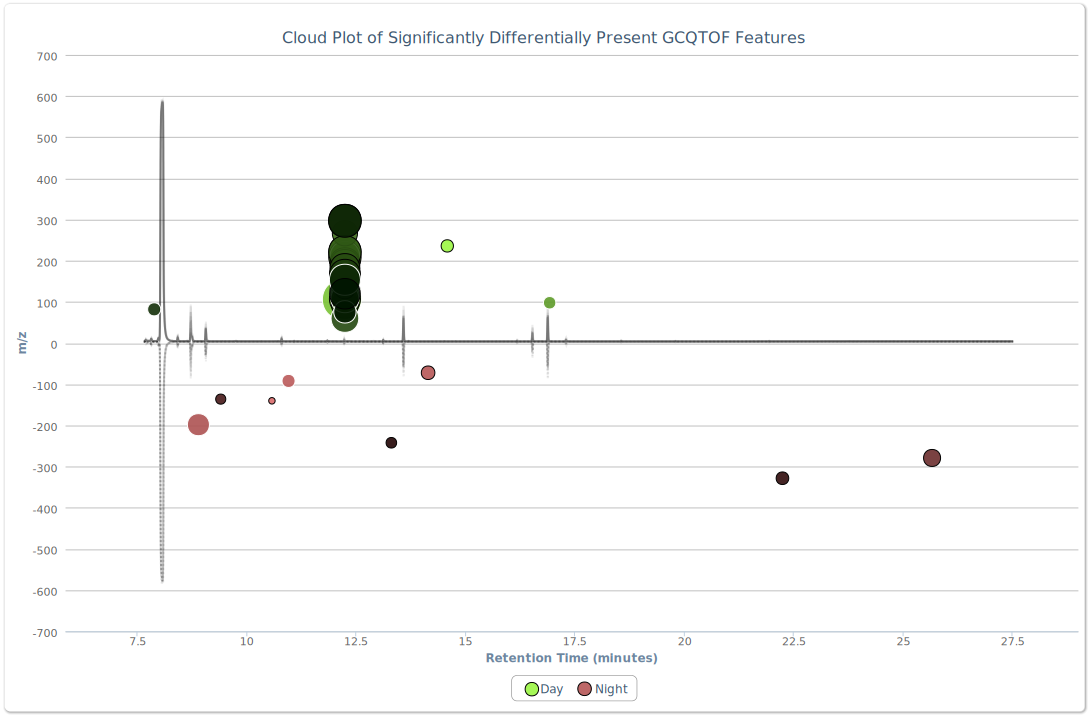
\includegraphics[width=\textwidth]{gcms_cloud_plots.pdf}
    \caption[GCQTOF Cloud Plot]{Cloud point showing for the GCQTOF analysis. 
    The radius of a given point reflected its fold change.
    Data is filtered to those 50 points with significantly 
different expression (FDR corrected P-value of 0.01 shown by 
depth of colour)}
    \label{fig:gcms_clouds}
\end{figure}


\begin{figure}
    \centering
    
\includegraphics{GCMS_metabolites.pdf}
    \caption[Plot of Identifiable GC-QTOF Metabolites]{Plot showing the
        fold change of the 23 putatively identifiable significantly
        differently present metabolites from GC-QTOF. 5 peaks
        were discarded after inspection of the EIC. 8 were discarded
    as there was no sensible annotation, 14 had no annotations.}
    \label{fig:gcms_metabolites}
\end{figure}



Only one metabolite putatively with a m/z matching glucose 
was identified with no significantly different expression.



\begin{figure}
    \centering
    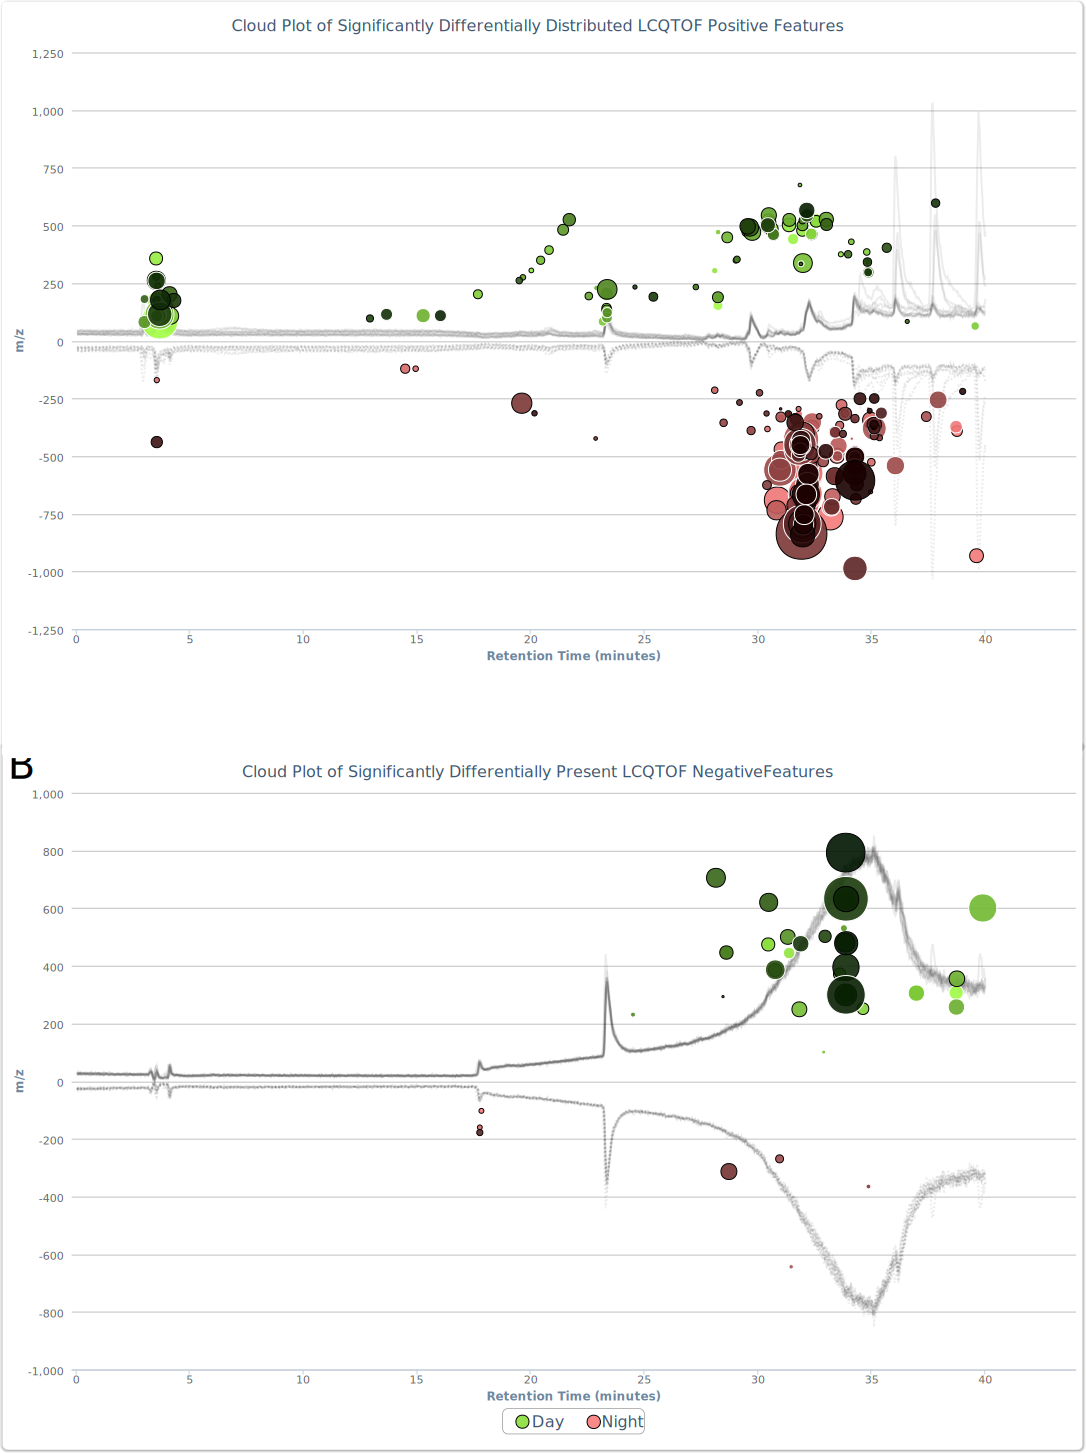
\includegraphics[width=\textwidth]{lcms_cloud_plots.pdf}
    \caption[LCQTOF Cloud Plots]{A: Positive 254,  B: 43}
    \label{fig:lcms_clouds}
\end{figure}


\begin{figure}
    \centering
    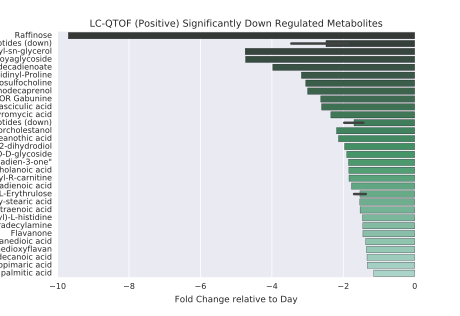
\includegraphics[width=\textwidth]{LCMS_pos_down_metabolites.pdf}
    \caption{Of the 254 positive significantly different present metabolites,
        19 were removed after manual inspection of peaks, 95 were removed due
    to having no METLIN hits}
    \label{fig:posqtofdown}
\end{figure}


\begin{figure}
    \centering
    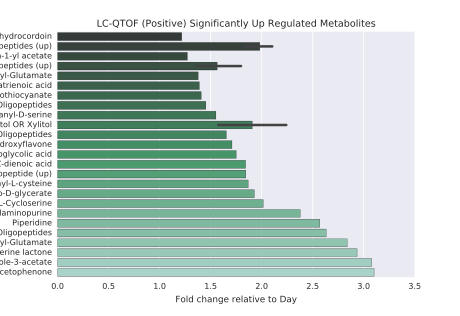
\includegraphics[width=\textwidth]{LCMS_pos_up_metabolites.pdf}
    \caption{Of the 254 positive significantly different present metabolites,
        19 were removed after manual inspection of peaks, 95 were removed due
    to having no METLIN hits}
    \label{fig:posqtofup}
\end{figure}


\begin{figure}
    \centering
    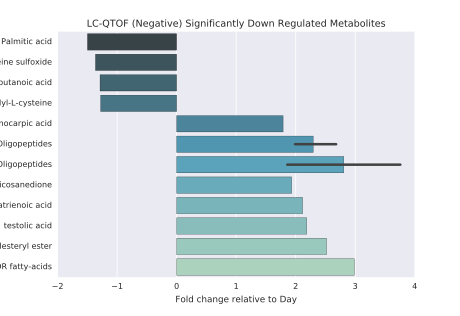
\includegraphics[width=\textwidth]{LCMS_neg_metabolites.pdf}
    \caption{Of the 43 positive significantly different present metabolites,
        3 were removed after manual inspection of peaks, 17 were removed due
    to having no METLIN hits}
    \label{fig:poslcqtof}
\end{figure}




Again one interesting peak is that of 
in negative
9.7 0.04846 DOWN with a fold vlaue of 9.7
putatively raffinose>? 503.1698  vs actual 503.169
    

\subsubsection{Targeted amino acid analysis}



\begin{figure}
    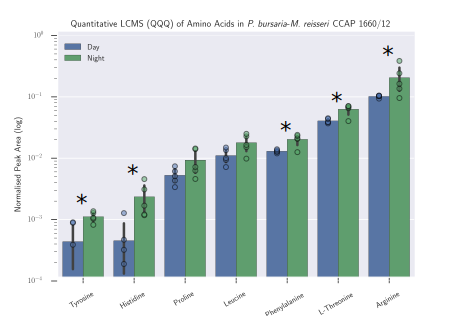
\includegraphics[width=\textwidth]{AA_LCMS.pdf}
    \caption[LCQQQ Quantitative Analysis of Amino Acids]{LC-QQQ analysis
        of amino acid abundances. Normalised Peak Areas 
        Calibration was conducted using Day1 and Night1 samples at two titrations, as well as Asn-Gln-Tryptamine and Sigma AA mixes
    Calibration and quantitative analysis failed for the following amino acids: 
Glutamic Acid, Tryptamine, Asparagine, Trpytophan, Isoleucine, Methionine, Valine, Serine, Glutamate, Glutamine, Aspartic acid, Cystein or Lysine.
Significant concentration differences between day and night (as determined via Welch's `\textit{t}' are indicated by an astrerisk.}
    \label{fig:amino_acids}
\end{figure}









\section{Discussion}

SEECER and K-mer abundance filtering may be mutually exclusive

\subsection{Quantification in MDA}

%Titrating ERCC spike-ins to level of single cell 
%It has become an increasingly established methodology to add RNA of known concentrations
%to extractions before library preparation to aid quantification
%and normalisation in downstream analysis. 
%Unforunately, there are no established methods for synthetic RNA spike-ins
%of known RNA concentrations (e.g. ERCC RNA standards \citep{Jiang2011}) with MDA
%sc-RNAseq. Specifically, standards would need to be carefully titrated to appropriate
%concentrations for single cell methods or they would overwhelm sequencing 


%therefore no such spike-ins were added. 

%    \item Just use SCT for transcript quantification i.e. map the SCT reads to a bulk derived \textit{de novo} assembly to generate counts (and is there a severe bias induced 
%        by the MDA amplification \citep{Liang2014}?)
%\end{itemize}  <>++
%However, MDA is prone to a degree of amplification bias \citep{Liang2014} which may be problematic in accurate inference of differential expression
%therefore, the suitability of MDA-based scRNA-Seq in particular will also need to be assessed.
%The only other published analysis of \textit{Paramecium bursaria} and its green algal endosymbionts by \citep{Kodama2014} largely
%side-stepped this issue by focussing on the analysis of host transcripts with and without the endosymbiont by filtering
%likely endosymbiont derived contigs from analysis using a crude MEGABLAST \(e^{-40}\) approach.
%Studies in related ciliates have demonstrated a high prevalence of alternative splicing events (5.2\% of genes in \textit{Tetrahymena
%    thermophila} for a single celled eukaryote \citep{Xiong2012}
%This paper also demonstrated the huge dynamic range of expression (and thus necessity of RNA-Seq over microarray approaches) in \textit{T. thermophila})
%with approximately 6 order of magnitude range \citep{Xiong2012}
%However, as both target species - host and endosymbiont are eukaryotes the complication of mRNA enrichment 
%is simplified due to the sufficiency of poly-A selection for this task (instead of rRNA depletion methods)
%Determining the necessary sequencing depth is also difficult.
%First achieved in \citep{Lao2009}





MDA has amplification bias with GC content - problem for PbMr \citep{Macaulay2014}


\subsection{All methods have limitations}

All the methods included here have major limitations.


Firstly, the identification and analysis of secreted and transporter proteins,
as well as the metabolic mapping is fundamentally reliant on the quality and completion
of the host and endosymbiont transcriptomes. 
Any transcript missing from these bins either due to failure to assemble, 
cryptic MDA biases, or erroneous binning into bins other than host or endosymbiont.

This incorporates the issues with false negatives. 




However, there is also the issue of false positives. 
This is especially important for the transporters where a minimal (as few as
a single amino acid) divergence is sufficient to convert them to non-transporting
sensor proteins \citep{Lalonde1999,Bianchi2010}.






Therefore, it is key that the functionally important 

blah has to be tested



\subsection{Limits of metabolomics analysis}

A more intelligent hypothesis testing than corrected unequal variance 't'-test
could be used such as Kurschke's Bayesian BEST algorithm \citep{Kruschke2013}.
This also has the advantage of a Bayesian inference which can be 
made robust to multiple comparisons without need for extensive correction
procedures by using standard multi-level approaches \citep{Gelman2009}.







\subsection{Potentially missing transporters}

One potential issue with the binning methodology used is
that any recently horizontally acquired host or endosymbiont 
transporters or other metabolic pathway proteins will have been misclassified
and potentially discarded into the ``food'' or ``unknown'' bin.

This is problematic as there is evidence for bacterially acquired 
hexose-phosphate transporters playing a key role in the 
establishment of primary plastid endosymbiosis \citep{Price2012,Karkar2015a}.

Ideally, future work could expand this transporter analysis over the 
``unknown'' and ``food'' binned sequences in combination with synteny
analyses using genomic sequences to investigate and identify
potential horizontally acquired transporters that may play a role.

Another issue with the binning approach used is the possibility
of totally novel transporter (and other proteins) not being classified
due to the dependence of the binning on homology to known sequences.
Therefore, totally novel proteins would not have been identified as 
``host'' or ``endosymbiont''.  Unfortunately, this problem 
could only properly be resolved with a thorough and robust 
draft quality genome for both host and endosymbiont which was outside
the scope of this analysis. 

The final source of obfuscation in an accurate analysis of this data
is that of host-endosymbiont gene transfer.  
This is well observed phenomenom that has resulted in the eventual loss
of the endosymbiotic in the majority of algal secondary endosymbiotic organelles
as genes are transferred to the host nucleus
\citep{Keeling2008a,Archibald2005,Keeling2004}.

It is unknown and difficult to determine to what extent the 
unusual nuclear dimorphism and germline sequestration of the host 
effect's the rate of this form of transfer. 

Fortunately, this binning method means that while some peptides
may have been falsely assigned to wrong bin all ``host'' and
``endosymbiont'' ORFs that were not either so novel they lacked
any homology to known proteins or were recently acquired from
bacteria were still included in this analysis. 

However, as some \textit{M. reisseri} and \textit{Chlorella} endosymbionts 
have been demonstrated as capable of free-living it is unlikely
that HGT has occurred between host and endosymbbiont as extensively
as that observed in established photosynthetic organelles. 


\subsection{Secretome}
Without knowledge of \textit{P. bursaria}'s intracellular trafficking
system it is not possible to easily infer which host peptides are secreted into
the PV.  For this reason, analysis of secreted proteins focussed on 
the endosymbiont bin as the secretion signal are generally better conserved
and established. 

Unfortunately, much as incorrect




\subsection{Metabolomics shows promise}

The pilot application of metabolomics demonstrated mixed results.
There was poor performance of mass

GC/MS failed for comprehensive profiling of carbohydrates.
Possibly due to miscalibration of the GC parameters or the capture 
paramters on the initial quadrupole.


All globally profiled metabolites required comprehensive validation
with a secondary mass spectrometry. 


The failure of accurate quantification in the second round
of MRM LC-QQQ spectrometry for the majority of amino acids 
is problematic.  However, this targeted approach still revealed
useful information regarding the relative abundance of amino.



Particularly, both the high concentration of arginine as well
as its significantly differential abundance between day and night
indicates that this amino acid may well form a major component of 
host provided nitrogen for \textit{M. reisseri}. This is in
concordance with previous findings suggesting 
the importance of this amino acid in the \textit{C. variabilis}
endosymbiosis \citep{Kato2006}.

Despite not have been implicated in previous analyses
as one of the key amino acid nitrogen sources, the identification
of both high quantities and differential abundant 
threonine and phenylalanine suggests that these
amino acids may play a role in the host-endosymbiont
barter system of \textit{P. busaria}-\textit{M. reisseri}.




This alternative behaviour suggests that the feeding experiment
results by \citep{Kato2006} and \citep{Kato2009} need 
to be re-evaluated for \textit{M. reisseri}. This also
adds further support to the diversity of endosymbiotic
relationships between \textit{P. bursaria} and its
various algal endosymbionts. 


Unfortunately, a failure to accurately quantify and calibrate
for several amino acids means this targeted metabolomic analysis
is incomplete.  Of particular interest, is the remaining 5 amino acids
implicated in \textit{C. variabilis} F36-ZK's endosymbiosis.








\subsection{Putatively novel role for Raffinose in endosymbiosis??}

galactinol + sucrose → myo-inositol + raffinos/



Unfortunately, the GCQTOF analysis failed to successfully
identify sugars in the 


Raffinose has been associated with cold shock in
\textit{Parachlorella kessleri} (formerly \textit{C. vulgaris}),
accumulating duing cold exposure and disappearing after return
to normal culture temperatures 

It is unclear if raffinose is a 
\citep{Salerno1989}


Raffinose and another Raffinose Family Oligosaccharide (RFO) 
stachyose are generated from sucosrse in gymnopserls during
the cold season \citep{Kandler1982}.

Raffinose has been found to inhibit growth under
isosomotic conditions in a \textit{C. vulgaris} 
\citep{Setter1979}.

Specifically, it has also been directly associated
with cryoprotection of thykaloid membranes \citep{Lineberger1980}.
And no chlorop targeting sequence though

But that doens't explain secretion.



Bacterial raffinose transport system?


In archaeplastida RFOs are related to stroage
and transport of carbon.  



What about trehalose?
sucrose?




phylogeny?





It does appear that the raffinose synthase is constitutively
expressed unless both light and dark conditions are exposed to cold stress.

Culture temperature was \(18\celsius\), so this is unlikely. 

Needs confirmed with qPCR. 





\subsection{Endosymbiont Nitrogen Metabolism}

One the balance of the evidence of significantly higher concentrations
of specific amino acids.

There is reason to believe that \textit{M. reisseri} CCAP 1660/12
endosymbiont displays a similar system to that of the Japanese
\textit{C. variabilis} F36-ZK strain in terms of amino acid usage. 

Intriguingly, the transcriptome reveals the presence of all sub-units
of the ABC-type branched amino-acid transporter not present in 
the other endosymbiotic green algae. 

Due to the huge range of possible 


While, NR and NiR are present in the \textit{M. reisseri} transcriptome
it is possible that these are non-functional like the mutants in 
NC64A and F36-ZK.




\section{Conclusion}

This preliminary analysis of host-endosymbiont metabolic integration 
has lead to some promising results.
Namely, discovering quantitative data supporting the mechanism by which
the host likely provides a nitrogen source to the endosymbiont. 
Specifically, 





Ultimately, the key finding from this analysis
is that \textit{M. reisseri} much like various strains of \textit{C. variabilis}
exhibit a range of adaptations to endosymbiosis and a given
host displays different behaviours. 







However, further work is needed to confirm both the role and loc

%\chapter{Endosymbiont Metabolic Analysis}
%
%http://www.sciencedirect.com/science/article/pii/S0888754312000250 - see this for analysis to copy \citep{Xie2012}

%
%
%Also of interest is the activity of fatty acid and amino acid biosynthesis in the endosymbiont.  This is because
%all well studied examples of primary of secondary plastids that have lost photosynthetic activity appear to maintain 
%essential roles in these and other areas of host metabolism.
%In all well-studied cases to date, the plastid itself is retained, as it is known to be the site of essential biochemical processes unrelated to photosynthesis, including fatty acid and amino acid biosynthesis (Waller and McFadden 2005; Barbrook et al. 2006; Mazumdar et al. 2006). \citep{Donaher2009}
%
%Additionally the comparison of photosynthetic \textit{Symbodinium} within their cindarian hosts in both autotrophic and mixotrophic conditions
%is of interest \citep{Xiang2015}
%Genes indeitnfied in paramecium tetaurelia involve din autogamy, reciliation and exocytosis respectively \citep{Arnaiz2010}
%Interestingly highly differentially expressed genes appear to have a lower rate of gene loss \citep{Arnaiz2010}
%Diffeq - single cell - technical noise important - must be quantifeid so it can be incorporated into 
%Low amount of RNA in single cell presents a major difficulity leading to unavoiable technicla noise \citep{Brennecke2013}
%Depth
%
%Unfortunately no ERCC because reasons
%http://www.nature.com/nmeth/journal/v10/n11/extref/nmeth.2645-S2.pdf
%
%
%
%
%mycosporina amino acids - shikimate pathway - protect agains UVR \citep{Sommaruga2009} (Shick and dunlap 2002)
%chlorella made MAA found in cilliates sonntag2007 
%Negative in p bursaria chlorella thoufgh summerer2009


%
%NMR was the traditional method - less sample preparation, rapid, nondestructive, high-throughput, robust
%
%LC - good for polar/apolar but bad frag, ion supression and small/very polar need special column
%GC - suited for apolar and volatiles - universal databank but needs high sample prep, derivatizatrion of polar and lots of frag
%

%It is also possible to use data-mining methods using existing 
%ontologies and annotations \citep{Lee2008}.


